%----------------------------------------------------------------------------------------
%	TITLE PAGE
%----------------------------------------------------------------------------------------
\documentclass[aspectratio=169]{beamer}
% use 16:9 in new slides!

\usepackage{tikz}
\usepackage{listings}
\usepackage{xcolor}
\usepackage{graphicx}
\usepackage{float}
\usepackage{tikz}
\usetikzlibrary{trees}
\usepackage{hyperref}
\usepackage{array}
\usepackage[skins]{tcolorbox}
\def\bpr#1#2{
\begin{tcolorbox}
[boxsep=.15cm,left=.2cm,right=.2cm,oversize,boxrule=0mm,
colback=green!55!blue!20!white!60,
colframe=red!50!yellow!50!white,
colbacktitle=blue!50, 
coltitle=black,enhanced,drop fuzzy shadow,
fonttitle=\bfseries,title=#1]
#2
\end{tcolorbox}
}

\def\bdef#1#2{
\begin{tcolorbox}
[boxsep=.15cm,left=.2cm,right=.2cm,oversize,boxrule=0mm,
colback=white!60,
colframe=red!50!yellow!50!white,
colbacktitle=green!50!yellow!60!gray, 
coltitle=black,enhanced,drop fuzzy shadow,
fonttitle=\bfseries,title=#1]
#2
\end{tcolorbox}
}

\def\bthe#1#2{
\begin{tcolorbox}
[boxsep=.15cm,left=.2cm,right=.2cm,oversize,boxrule=0mm,
colback=white!60,
colframe=red!50!yellow!50!white,
colbacktitle=red!52, 
coltitle=black,enhanced,drop fuzzy shadow,
fonttitle=\bfseries,title=#1]
#2
\end{tcolorbox}
}

\def\tcb#1{
\begin{tcolorbox}
[boxsep=.15cm,left=.2cm,right=.2cm,oversize,boxrule=0mm,
colback=white!60,
colframe=red!50!yellow!50!white,
colbacktitle=red!50!yellow!50!white, coltitle=black,enhanced,drop fuzzy shadow,]
#1
\end{tcolorbox}
}



\definecolor{UMBlue}{RGB}{5,32,103}
\definecolor{UMYellow}{RGB}{255,216,0}
%\usetheme{Madrid}
\setbeamertemplate{headline}{
  \leavevmode%
  \begin{minipage}{0.75\paperwidth}
  \vspace{1.2ex}\hspace{-0.245\paperwidth}
  \resizebox{\paperwidth}{3ex}{
    \tikz{
      \fill [color=UMBlue] (0,0) rectangle (10, 0.13);
      \fill [color=UMYellow] (0,-0.1) rectangle (10, -0.18);
    }
  }
  \begin{beamercolorbox}[wd=\linewidth,ht=2.5ex,dp=1.125ex]{section}
    \insertsubsectionnavigationhorizontal{\linewidth}{}{Slide \insertpagenumber}
  \end{beamercolorbox}
  \end{minipage}
  \begin{minipage}{0.23\paperwidth}
  \hspace{0.2em}
  
\includegraphics[width=\linewidth]{img/logo.png}
  \end{minipage}
}

\setbeamercolor{title}{fg=UMBlue}
\setbeamercolor{frametitle}{fg=UMBlue}
\setbeamercolor{structure}{fg=UMBlue}

\title[Course number]{Git Workshop} 
\author[]{TechJI}
\institute[UMJI-SJTU]
{
	University of Michigan - Shanghai Jiaotong University
	\\\medskip
	Joint Institute
}
\date{2025.05}
%----------------------------------------------------------------------------------------
%	Highlight the title of the current section
%----------------------------------------------------------------------------------------
\AtBeginSection[]
{
  \begin{frame}
    \frametitle{Table of Contents}
    \tableofcontents[currentsection]
  \end{frame}
}



\begin{document}
\maketitle
\begin{frame}
  \frametitle{Table of Contents}
  \tableofcontents
\end{frame}

\section{Introduction}
\subsection{Shell}
\begin{frame}
  \frametitle{What is a Shell?}

  A \textbf{shell} is a text-based interface for interacting with the operating system.

  \vspace{0.7em}
  It lets you run programs, navigate files, and automate tasks by typing commands.

  \vspace{1em}
  \textbf{Common shells:}
  \begin{itemize}
    \item Zsh — default on macOS
    \item Bash — default on most Linux systems
    \item PowerShell — default on Windows
  \end{itemize}
\end{frame}


\begin{frame}
  \frametitle{What You Can Do With the Shell}

  \begin{columns}[T] 
    \column{0.5\textwidth}
    \begin{minipage}[t]{\linewidth}
      \textbf{Basic commands (see cheat sheet):}
      \begin{itemize}
        \item Navigation: \texttt{cd}, \texttt{ls}, \texttt{pwd}
        \item Files: \texttt{touch}, \texttt{mkdir}, \texttt{mv}, \texttt{rm}, \texttt{cp}
        \item Viewing: \texttt{cat}, \texttt{less}, \texttt{head}, \texttt{tail}
      \end{itemize}
    \end{minipage}

    \column{0.5\textwidth}
    \begin{minipage}[t]{\linewidth}
      \textbf{Shell has its own scripting language:}

      \vspace{0.5em}
      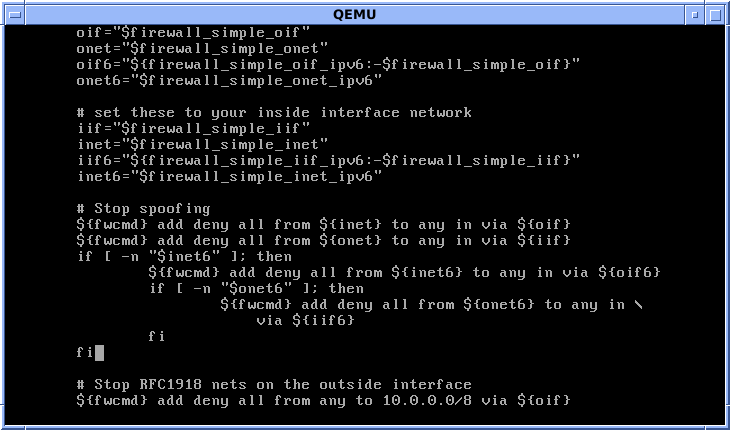
\includegraphics[width=\linewidth]{img/shell-scripting1.png}
    \end{minipage}
  \end{columns}
\end{frame}


\begin{frame}
  \frametitle{Exercise}
  \textbf{Tasks:}
  \begin{enumerate}
    \item Go to your Desktop directory
    \item Create a folder called \texttt{test}
    \item Inside that folder, create a new file named \texttt{ex1.c}
  \end{enumerate}

  \vspace{1em}
  \textbf{Hint:}
  Use: \texttt{ls}, \texttt{cd}, \texttt{touch}

\end{frame}

\subsection{Git}
\begin{frame}
  \frametitle{What is Git?}

  Git is a distributed version control system. It keeps a full history of your project and allows you to:
  \begin{itemize}
    \item Track changes over time
    \item Go back to any previous state
    \item Work in parallel via branches
    \item Merge contributions from others
  \end{itemize}

  \vspace{1em}
  Unlike services like Feishu Docs, Git gives you full control and works offline.
\end{frame}


\begin{frame}
  \frametitle{Why Use Git?}

  \begin{itemize}
    \item Prevent messy filenames like \texttt{report-final-fixed-v3-real.c}
    \item Add different features simultaneously without breaking the main project
    \item Collaborate with others without conflicts
    \item Manage not only code, but also papers, configs, and notes
  \end{itemize}

  \vspace{1em}
  Git isn’t just for teams — it’s a useful tool even if you work alone.
\end{frame}


\begin{frame}
  \frametitle{How Do We Use Git?}

  Git is installed locally — see the \texttt{installation\_git} guide in the repo.

  \vspace{1em}
  Once installed, you can use Git in different ways:
  \begin{itemize}
    \item In the terminal (CLI) — direct and powerful
    \item With tools like \texttt{lazygit} (TUI) — text-based UI in the terminal
    \item In graphical interfaces (GUI) — like GitHub Desktop or inside VS Code
  \end{itemize}

  \vspace{1em}
  Git also works with remote platforms like GitHub and Gitea — both are based on Git.  
  They let you back up projects online, share with others, and collaborate more easily.
\end{frame}
  

\section{Basic Git Commands}

\begin{frame}
  \frametitle{Git Setup: init and clone}

  \textbf{Initialize a repository}
  \begin{itemize}
    \item Creates a Git project in the current folder.
    \item Adds a hidden \texttt{.git} directory to track changes.
  \end{itemize}
  \vspace{0.3em}
  \texttt{git init}

  \vspace{1em}
  \textbf{Clone an existing repository}
  \begin{itemize}
    \item Copies all files and full version history from a remote project.
    \item You can now contribute locally.
  \end{itemize}
  \vspace{0.3em}
  \texttt{git clone <repository-url>}

\end{frame}

\begin{frame}
  \frametitle{Saving Changes: add and commit}

  \textbf{Stage changes}
  \begin{itemize}
    \item Choose which changes you want to include in your next commit.
  \end{itemize}
  \vspace{0.3em}
  \texttt{git add <file>}

  \vspace{1em}
  \textbf{Create a snapshot}
  \begin{itemize}
    \item Save staged changes with a message.
    \item This becomes part of the project's version history.
  \end{itemize}
  \vspace{0.3em}
  \texttt{git commit -m "your message"}

  \vspace{1em}
  Tip: Commit frequently, with clear messages.
\end{frame}

\begin{frame}
  \frametitle{Remote Sync: push and pull}

  \textbf{Upload local changes}
  \begin{itemize}
    \item Send your commits to a remote repository (e.g., GitHub, Gitea).
  \end{itemize}
  \vspace{0.3em}
  \texttt{git push}

  \vspace{1em}
  \textbf{Download new changes}
  \begin{itemize}
    \item Fetch and merge new commits from the remote repository into your current branch.
  \end{itemize}
  \vspace{0.3em}
  \texttt{git pull}

  \vspace{1em}
  Tip: Always pull before pushing to avoid conflicts.
\end{frame}


\begin{frame}
  \frametitle{Switching Branch: checkout}

  \textbf{Switch to another branch}
  \begin{itemize}
    \item Move to a different line of development.
  \end{itemize}
  \vspace{0.3em}
  \texttt{git checkout <branch-name>}

  \vspace{1em}
  \textbf{Restore a file}
  \begin{itemize}
    \item Undo changes to a file and bring it back to the last committed version.
  \end{itemize}
  \vspace{0.3em}
  \texttt{git checkout -- <file>}

  \vspace{1em}
  Note: Git 2.23+ supports \texttt{git switch} and \texttt{git restore} as clearer alternatives.
\end{frame}


\begin{frame}
  \frametitle{Merge Conflicts}

  \textbf{What is a merge conflict?}
  \begin{itemize}
    \item Happens when Git can't auto-combine changes from two sources.
    \item Often caused by editing the same lines in different commits.
  \end{itemize}

  \vspace{1em}
  \textbf{When does it happen?}
  \begin{itemize}
    \item \texttt{git merge} or \texttt{git pull} introduces conflicting edits
    \item Someone else pushed to the same branch and you didn’t pull first
  \end{itemize}

  \vspace{1em}
  Git pauses and asks you to fix the conflict before continuing.
\end{frame}


\begin{frame}
  \frametitle{Resolving Conflicts: Manual Editing}

  \textbf{Step 1: Open the conflicted file}  
  Git marks the conflict like this:

  \texttt{<<<<<<< HEAD} \\
  \texttt{your version} \\
  \texttt{=======} \\
  \texttt{their version} \\
  \texttt{>>>>>>> branch-name}

  \vspace{1em}
  \textbf{Step 2: Manually edit}
  \begin{itemize}
    \item Choose which code to keep (or combine)
    \item Delete conflict markers
  \end{itemize}

  \vspace{1em}
  \textbf{Step 3: Save and confirm}
  \texttt{git add <file>} \\
  \texttt{git commit}

\end{frame}


\begin{frame}
  \frametitle{Resolving Conflicts: Git Commands (Optional)}

  \textbf{These tools can help, but use with care:}

  \vspace{0.5em}
  \texttt{git diff} — See differences between conflicting versions

  \vspace{0.5em}
  \texttt{git merge --abort} — Cancel merge and return to previous state

  \vspace{0.5em}
  \texttt{git checkout -- <file>} — Discard changes and restore last committed version

  \vspace{0.5em}
  \texttt{git reset --mixed} — Unstage and reset to last commit

  \vspace{1em}
  Start with manual fixes. Use commands if you're more confident.
\end{frame}


\begin{frame}
  \frametitle{Never Use \texttt{--force}}

  \begin{columns}
    \begin{column}{0.6\textwidth}
      \texttt{git push --force} can permanently delete others' work.

      \vspace{0.6em}
      \textbf{Why it's dangerous:}
      \begin{itemize}
        \item Overwrites history on shared branches
        \item Causes teammate data loss
        \item Breaks collaboration workflows
      \end{itemize}

      \vspace{0.6em}
      AI tools (e.g. GitHub Copilot, ChatGPT) may suggest it blindly.\\
      Unless you're working solo and fully understand it, don't use \texttt{--force}.
    \end{column}

    \begin{column}{0.4\textwidth}
      
\includegraphics[width=\textwidth]{img/git-force1.png}
    \end{column}
  \end{columns}
\end{frame}








  
\section{Non-CLI Interfaces}
\subsection{VS Code Extension}
\subsection{LazyGit(Optional)}



\end{document}
